\section{Experiments and results}

With the tools and methodology defined in the previous sections, we can now proceed to the experiments. Each run is determined by its configuration, that can be divided into the following categories:

\begin{itemize}
\item \textbf{Feature set}: Determinates the encoding of the position, and thus the number of inputs of the model. It conditions which patterns the network can learn.

\item \textbf{Network architecture}: The size of each layer in the network. The first layer is the feature transformer, and its size roughly determinates how many patterns the network can learn. The following two layers should be tiny due the NNUE architecture.

\item \textbf{Dataset}: blabla

\item \textbf{Training method}: Can choose to use either Stockfish evaluations or PQR triplets. This determinates the format of the samples as well as the loss function. Most experiments will train using Stockfish evaluations.

\item \textbf{Training hyperparameters}: The usual machine learning hyperparameters for training, such as batch size, learning rate and scheduler.
\end{itemize}

To assess the performance of a run or to compare a set of runs, the following indicators can be used:

[hablar de que hay runs particulares que miden otras cosas pero estas son generales]

\begin{itemize}
\item \textbf{Puzzle accuracy}:
\item \textbf{Relative ELO performance}:
\item \textbf{Inference performance (infs/s)}:
\item \textbf{Training time (not important, one time)}:
\end{itemize}


The experiments are all run in the same hardware: Intel 14900K CPU for dataset generation, batching and evaluation, and a single NVIDIA RTX 4090 24GB GPU for training.

\subsection{Baselines}

The objective is to find good baselines to compare the experiments that will follow.

P and KP
Network size?
Inference time?

a partir de cierto punto al loss le cuesta bajar pero las otras metricas siguen mejorando, asi que sigo entrenando

hacer side by side de Piece y KingPiece:

matriz con dos ejes: batch size y L1 size. con colores?

\begin{figure}[H]
\centering
\makebox[\textwidth]{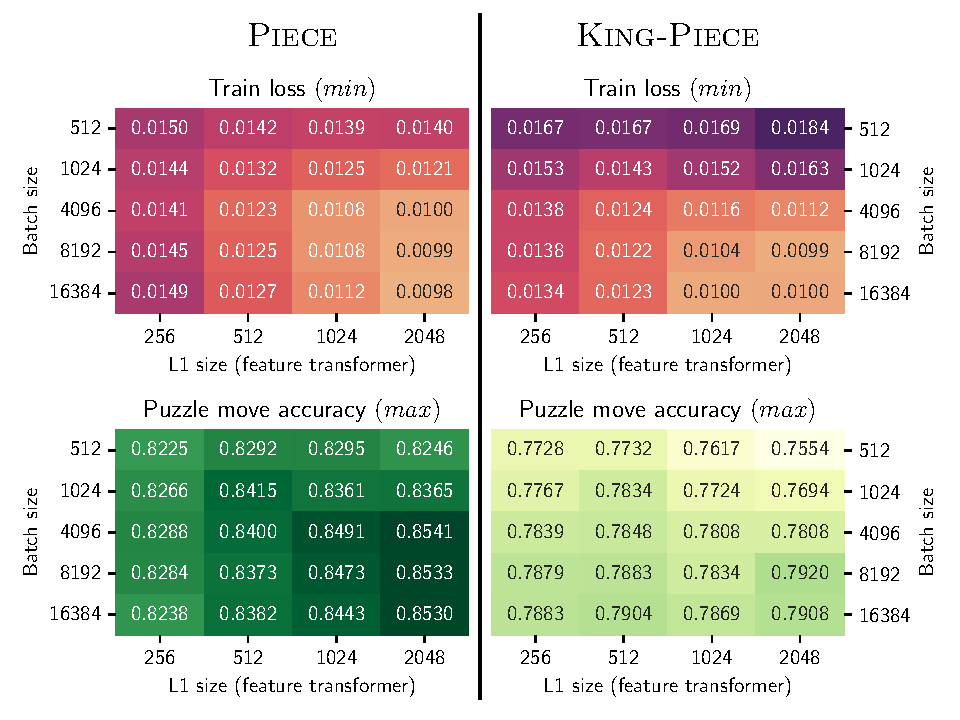
\includegraphics[width=\textwidth]{./dynamic/baselines_comparison.pdf}}
\caption{ASDASDASD}
\label{fig:asdasdasd}
\end{figure}


\newpage
\subsection{Axis encoding} % relevance

\newcommand{\axisarrows}[1]{\parbox{0.7cm}{\includegraphics[height=0.7cm]{../assets/arrows/#1.pdf}}}

In this first experiment, I will explore different positional encodings for the pieces on the board, combining the available axes. The canonical \featureset{Piece} feature set encodes each piece's position using the square it is located. Note that this is the same thing as encoding the position for a piece $P$ as $\featureset{File}_{P} \times \featureset{Rank}_{P}$. So the position of each piece is determined using the vertical (across ranks) and horizonal (across files) axes. There are los of ways to index the board, but I will stick to the most common axes:

\begin{table}[H]
\centering
\begin{tabular}{cccc}
\axisarrows{H} & \axisarrows{V} & \axisarrows{D1} & \axisarrows{D2} \\
Horizontal & Vertical & Diagonal 1 & Diagonal 2 \\
(across files) & (across ranks) &  & 
\end{tabular}
\end{table}

a proposito se parecen mucho a los movimientos de las piezas...


\begin{table}[H]
\centering

\newcommand{\rolecolor}{$\times$ $\featureset{Role}_{P} \times \featureset{Color}_{P}$}

\begin{tabular}{@{} ccccc @{}} \toprule
\bf Depiction & \bf Feature set & \multicolumn{2}{c}{\makecell{\bf Definition\\for every piece $P$ in the board}} & \bf \makecell{\# of\\features} \\
\toprule
\axisarrows{HV} & \featureset{HV (Piece)} & $\featureset{File}_{P} \times \featureset{Rank}_{P}$ & \rolecolor & 768 \\
\midrule
\axisarrows{H} $\oplus$ \axisarrows{V} & \featureset{H+V} (\featureset{Compact}) & $(\featureset{File}_{P} \oplus \featureset{Rank}_{P})$ & \rolecolor & 192 \\
\midrule
\axisarrows{D1D2} & \featureset{D1D2} &  $\featureset{Diag1}_{P} \times \featureset{Diag2}_{P}$ & \rolecolor & 2700 \\
\midrule
\axisarrows{D1} $\oplus$ \axisarrows{D2} & \featureset{D1+D2} & $(\featureset{Diag1}_{P} \oplus \featureset{Diag2}_{P})$ & \rolecolor & 360 \\
\midrule
\axisarrows{HV} $\oplus$ \axisarrows{D1D2} & \featureset{HV+D1D2} & \makecell{$(\featureset{File}_{P} \times \featureset{Rank}_{P}$ $\oplus$ \\ $\featureset{Diag1}_{P} \times \featureset{Diag2}_{P})$} & \rolecolor & 3468 \\
\midrule
\makecell{\axisarrows{H} $\oplus$ \axisarrows{V} $\oplus$ \\ \axisarrows{D1} $\oplus$ \axisarrows{D2}} & \featureset{H+V+D1+D2} & \makecell{$(\featureset{File}_{P} \oplus \featureset{Rank}_{P}$ $\oplus$ \\ $\featureset{Diag1}_{P} \oplus \featureset{Diag2}_{P})$} & \rolecolor & 552 \\
\midrule
\axisarrows{HD1} $\oplus$ \axisarrows{VD2} & $\featureset{HD1} \oplus \featureset{VD2}$ & \makecell{$(\featureset{File}_{P} \times \featureset{Diag1}_{P}$ $\oplus$ \\ $\featureset{Rank}_{P} \times \featureset{Diag2}_{P})$} & \rolecolor & 2880 \\
\midrule
\axisarrows{VD1} $\oplus$ \axisarrows{HD2} & $\featureset{VD1} \oplus \featureset{HD2}$ & \makecell{$(\featureset{Rank}_{P} \times \featureset{Diag1}_{P}$ $\oplus$ \\ $\featureset{File}_{P} \times \featureset{Diag2}_{P})$} & \rolecolor & 2880 \\
\bottomrule
\end{tabular}

\caption{Axis encoding feature sets}
\label{tab:axis_encoding}
\end{table}

\vspace{2cm}

z
Mirar si sacando informacion en un eje mejora/empeora. La idea es ver si la informacion vertical es mas importante que la horizontal. Ver si incluir diagonales ayuda.

\subsection{Symmetry}

Medir el impacto de agregar simetría al fs. Red mas chica, inf mas rapida, mejor perf?

\featureset{Half-Relative(H|V|HV)King-Piece}?

\subsection{Piece movement}

Intentar capturar los patrones que se ven en P, asi se pueden reconocer patrones mas complejos.

\featureset{Piece-Move}

Bad perf.

\subsection{Statistical features}

Define \featureset{k-Piece-Piece}

\featureset{King-Piece} is a subset of \featureset{Piece-Piece}.

Top P

Hacer un subset de \featureset{PP} (589824).

\begin{itemize}
\item Destilar?
\item Probar si es lo mismo quedarse con el TOP K de las mas comunes o con las que dice el performance.
\item Catboost? PCA?
\end{itemize}

\subsection{Human behavior}

PQR human behaviour. Medir estilo Maia. comparar? no va a ser tan bueno.




% -----------------
hablar del tradeoff de los feature sets, la primera capa, y demás

vertical and horizontal data, probar dataset sin info vertical u horizonal / ambos y ver que pasa
ver si agregar capas posteriores ayuda o no "layer layers small increase in perf"

measure updates per move average and refreshes average per FS



\subsection{Active neurons}

medir si hay feature sets que no usen neuronas, que esto disparo el uso de HalfTopK

average number of features enabled by feature set (cantidad y porcentaje)



